\documentclass[a4paper, french]{article}

%% Language and font encodings
\usepackage{babel}
\usepackage[utf8]{inputenc}
\usepackage[T1]{fontenc}

%% Sets page size and margins
\usepackage[a4paper,top=3cm,bottom=2cm,left=2.5cm,right=2.5cm,marginparwidth=1.75cm]{geometry}
\usepackage{multicol}
\usepackage{parskip}


%% Useful packages
\usepackage{amsmath}
\usepackage{amsfonts}
\usepackage{graphicx}
\graphicspath{ {images/} }
\usepackage[colorinlistoftodos]{todonotes}
\usepackage[colorlinks=true, allcolors=blue]{hyperref}
\usepackage{float}

\title{ivegotmail -- compte-rendu --\\ Classification Binaire de Spams}
\author{Ben Kirane Malik, Mouhoubi Fatima}

\begin{document}
\maketitle
%\begin{multicols}{2}
\setlength{\parskip}{0.1in}
\setlength{\parindent}{15pt}

\begin{abstract}
Nous nous int\'eressons au probl\'eme de classification d'une base de courriers \'el\'ectroniques (emails). Nous souhaitons \`a partir du corps d'un email savoir s'il s'agit d'un spam ou non. Il s'agit d'inf\'erer cette connaissance \`a partir d'un corpus d'emails avec une approche bas\'ee sur les probabilit\'es (relation de Bayes). Cette approche est  pr\'esent\'ee en premi\`ere partie. L'objet de ce compte-rendu est ensuite d'\'etudier diff\'erentes mod\'elisations avec des descriptions enrichies pour r\'epondre au probl\'eme de classification.
\end{abstract}

\section{Classifieur par\\Inf\'erence Bay\'esienne}
Dans cette partie, pour inf\'erer \`a partir des distributions de probabilit\'es estim\'ees dans la phase d'apprentissage si un email est un spam ou non, nous illustrerons une solution \'a cette probl\'ematique  avec un mod\'ele tr\`es simple.  
Nous travaillerons tout le long sur deux phases distinctes : la phase d'apprentissage et la phase d'\'evaluation ou de pr\'ediction pour discuter de la qualit\'e du mod\`ele choisis.

Il est naturel de s'int\'eresser \`a la description d'un email, description que nous noterons $D(x)$ ou $\hat{x}$, s'il s'agit d'un spam nous lui associeront une \'etiquette de valeur $+1$, sinon de valeur $-1$. 
Au d\'epart avec un ensemble d'apprentissage $E=\left\{(x,y), y\in \left\{-1,+1\right\}\right\}$ et formellement, nous cherchons une application $f_{\Theta(E)}$  (classifieur), telle que pour tout email $x$ non n\'ecessairement dans $E$, $f_{\Theta(E)}(x)$ soit la classe de $x$. 

La phase d'apprentissage est donc la phase o\`u l'on estimera le mod\`ele  $\Theta(E)$ par inf\'erence sur $E$ et la phase d'\'evaluation est la phase o\'u on calcul l'image de $f_{\Theta(E)}$ pour un ensemble d'emails.

Nous consid\'erons deux variables al\'eatoires:
\begin{enumerate}
\item $X$ prendra les valeurs possibles des descriptions pour un email
\item $Y$ vaut $+1$ ou bien $-1$ selon qu'il s'agit respectivement d'un spam ou non.
\end{enumerate}

Notre approche est probabiliste : on souhaite par intuition conna\^itre les distributions 
\label{eq:estimation}
\begin{equation}P(Y=y|X=\hat{x}),\ \ y\in\{-1,+1\}\end{equation}
et pouvoir les comparer pour esp\'erer ensuite pr\'edire si $D^{-1}(\hat{x})$ (l'email d\'ecrit par $\hat{x}$) est un spam ou encore si l'application $\hat{f}_E\colon Im(X)\rightarrow \{+1,-1\}$ apprise avec la description $D$ indique pour un email $x$ sa classe simplement par le calcul $\hat{f}_E[ D(x)]$.

La fronti\`ere de d\'ecision peut se cacluler en utilisant la relation de Bayes sur les probabilit\'es conditionnelles \eqref{eq:estimation}
\begin{align}
\label{eq:estimation_spam}
\frac{P(X=\hat{x}|Y=+1)P(Y=+1)}{P(X=D(x))}
- \frac{P(X=\hat{x}|Y=-1)P(Y=-1)}{P(X=D(x))}=0
\end{align}

\eqref{eq:estimation_spam} est l'estimation qu'un email d\'ecrit par $\hat{x}$ est un spam (resp. n'est pas un spam) pond\'er\'ee par le ratio entre le nombre de spam (resp. non spam) et des emails de m\^eme description.

Nous consid\'erons la description $D\colon x\mapsto l(x)$ 
tel que $l(x)\in \mathbb{N}$ est la longeur du corps d'un email. 
Nous estimons, pour cette description, \'etant donn\'e une classe 
sur l'ensemble d'apprentissage, en comptant le nombre d'emails 
pour chaque description apparue lors du parcours de l'ensemble d'apprentissage. 
Il s'agit d'utiliser l'estimateur de fr\'equence pour la probabilit\'e 
$P(X=D(x)|Y=y)$. Puis nous estimons la distribution de $P(Y=y)$ parceque 
l'ensemble d'apprentissage est fini. 
La distribution sur la classe des spams de notre estimateur est 
repr\'esent\'ee sur la F\textsc{igure} \ref{fig:histo1spam}.

\begin{figure}[h!]
\begin{center}
    \caption{Estimation sur la longueur des spam}
    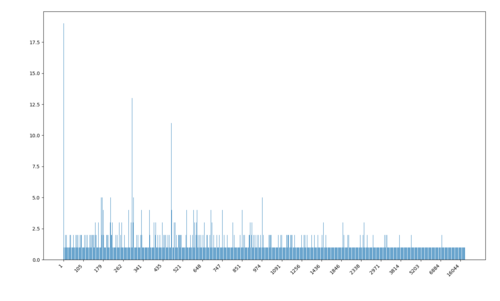
\includegraphics[width=13cm]{histo}
\end{center}
\label{fig:histo1spam}
\end{figure}

%\end{multicols}
\end{document}
